% !TEX encoding = UTF-8 Unicode
% !TEX TS-program = LilyPond-Book
\documentclass[12pt]{book}
\usepackage{pdfpages}
\usepackage[paperheight=11in,paperwidth=17in,margin=1in]{geometry}
\usepackage{multicol}
\usepackage{graphicx}
\setlength{\columnsep}{3cm}
\date{fdch}
\title{a.le.a}
\author{score}
\setcounter{secnumdepth}{-1}
\usepackage{titlesec}
\titlespacing\section{0pt}{12pt plus 4pt minus 2pt}{0pt plus 2pt minus 2pt}
\titlespacing\subsection{0pt}{12pt plus 4pt minus 2pt}{0pt plus 2pt minus 2pt}
\titlespacing\subsubsection{0pt}{12pt plus 4pt minus 2pt}{0pt plus 2pt minus 2pt}
\usepackage{scrlayer}
\DeclareNewLayer[
    foreground,
    %textarea,% use only the textarea
    contents={%
      \parbox[b][\layerheight][c]{\layerwidth}
        {\centering this page is intentionally left blank}%
    }
  ]{blankpage.fg}
\DeclarePageStyleByLayers{blank}{blankpage.fg}


\begin{document}
\maketitle
\begin{multicols}{2}
\section{performance notes}
\subsection{transposed score}
\input{../../../../reference/transposed.txt}
\subsection{dynamics}
\input{../../../../reference/dynamics.txt}
\subsection{pitches}
\input{../../../../reference/pitches.txt}
\subsection{rhythm}
\input{../../../../reference/rhythm.txt}
\subsection{tempo}
\input{../../../../reference/tempo.txt}
\columnbreak
\section{program notes}
\input{../../../../reference/program.txt}
\end{multicols}
\newpage
\section{notation}
\begin{multicols}{3}
\subsection{flute}
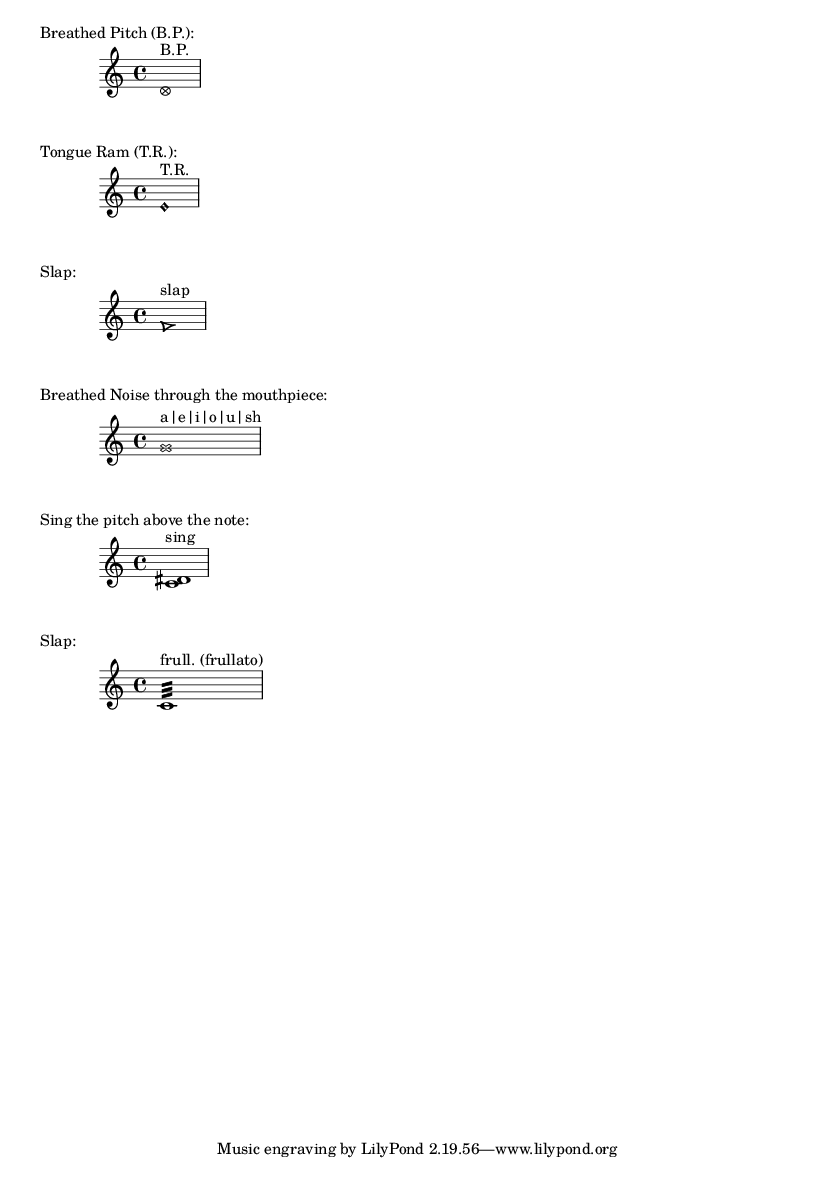
\includegraphics[scale=0.7, clip, trim=0 2cm 10cm 0 ]{../../../../reference/flute-notation.png}
\subsection{clarinet}
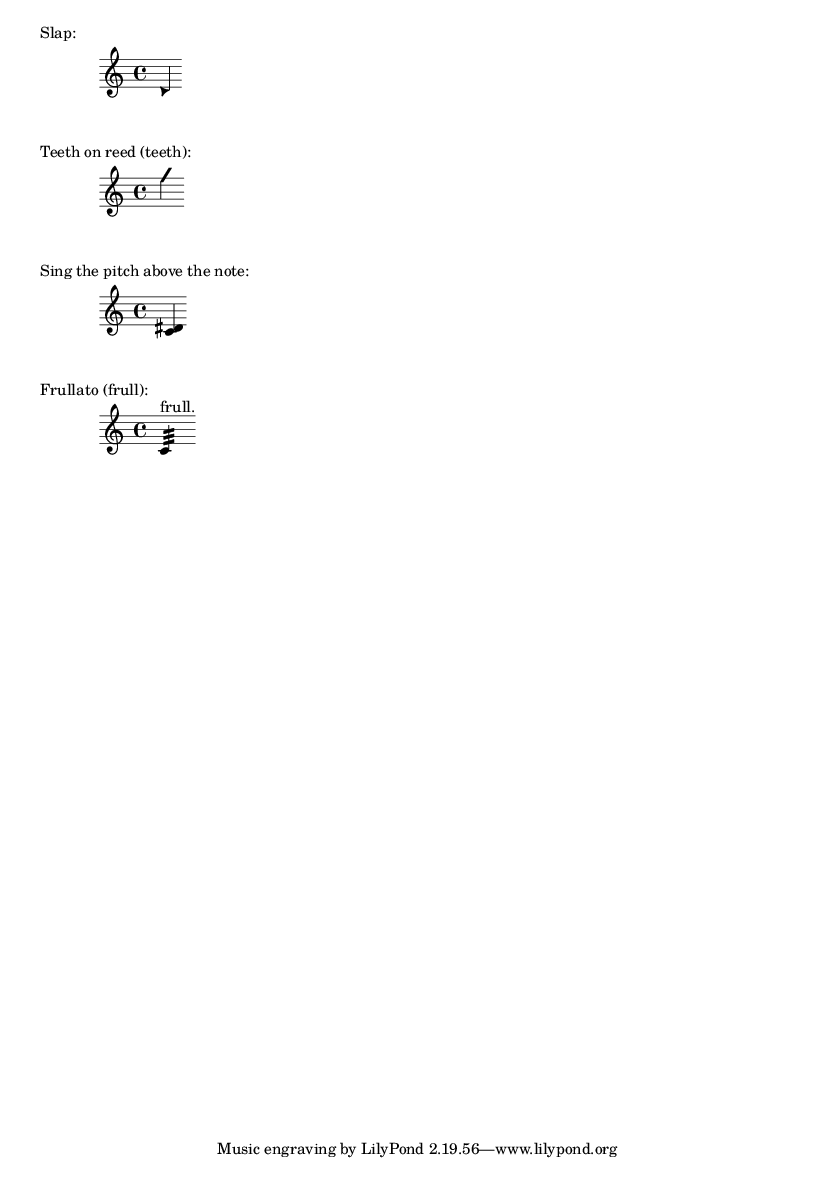
\includegraphics[scale=0.7, clip, trim=0 2cm  10cm 0 ]{../../../../reference/clarinet-notation.png}
\subsection{percussion}
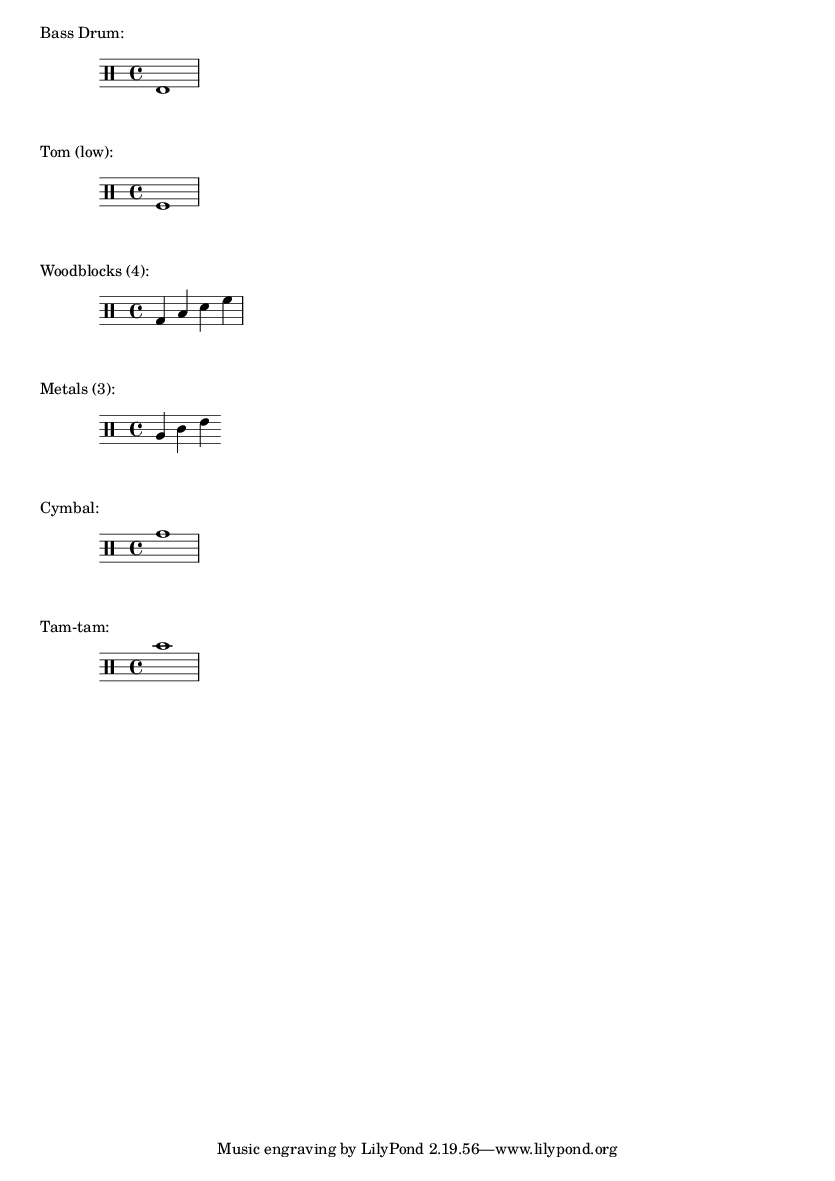
\includegraphics[scale=0.7, clip, trim=0 2cm 10cm 0 ]{../../../../reference/perc-setup.png}
\end{multicols}
\newpage
\null
\thispagestyle{blank}
\newpage
\end{document}